%!TEX root = ../dissertation_vkslm.tex

\chapter{Experimental Evaluation}\label{ch:exp}

In order to evaluate the quality of the synthetic signatures generated by our system we follow the same protocol presented on the work of Diaz \cite{diaz2014generation}. Namely we use a state-of-the-art off-line verification system and a dataset comprising both on-line and off-line signatures in order to train the verification system to evaluate the synthetic signatures.

The main idea of the experiments is to measure the quality of the synthetic signatures taking into account an off-line verification system performance. The questions raised on the experiments are \begin{inlinelist}
  \item is the synthetic signatures system performance similar to the real off-line signatures performance?
  \item is the performance even if the enrollment protocol changes?
  \item is it feasible to increase the number of samples at the enrollment stage with synthetic signatures? 
\end{inlinelist}



\section{Off-line signature verification system}
The system used for the evaluation of the real and synthetic signatures is a Linear SVM classifier and is based on a state of the art feature extraction approach  \cite{hafemann2017learning}. The feature extraction system \footnote{https://www.etsmtl.ca/Unites-de-recherche/LIVIA/Recherche-et-innovation/Projets/Signature-Verification} use ideas from transfer learning and multi-task learning to learn features using Convolutional Neural Networks (CNN).

SVMs represent a special class of linear classifiers. In order to classify a pattern as
belonging to one of two classes, an SVM constructs a hyperplane in the feature space,
such that it maximally separates the margin between the two classes. For this reason,
SVMs are also referred to as maximum margin classifiers 

\section{Evaluation Database}


The evaluation experiments were carried out on the BiosecurID
database \cite{biosecurid}. This multimodal database comprises on-
line and off-line signatures of 400 users. Signatures were
captured using a special digital inking pen on a paper placed
over a digitizing tablet. This way, both versions, on-line and
off-line, of the exact same real signature were acquired at
the same time. The database was captured in 4 sessions
distributed over 4 months. Each subject signed 4 times and
forged 3 signatures, thus leading to 4x4 = 16 genuine
samples and 3x4 = 12 skilled forgeries. The performance
of the real and synthetic signatures is evaluated on a subset
of 132 subjects.
\begin{figure*}[!htb]
	\centering
	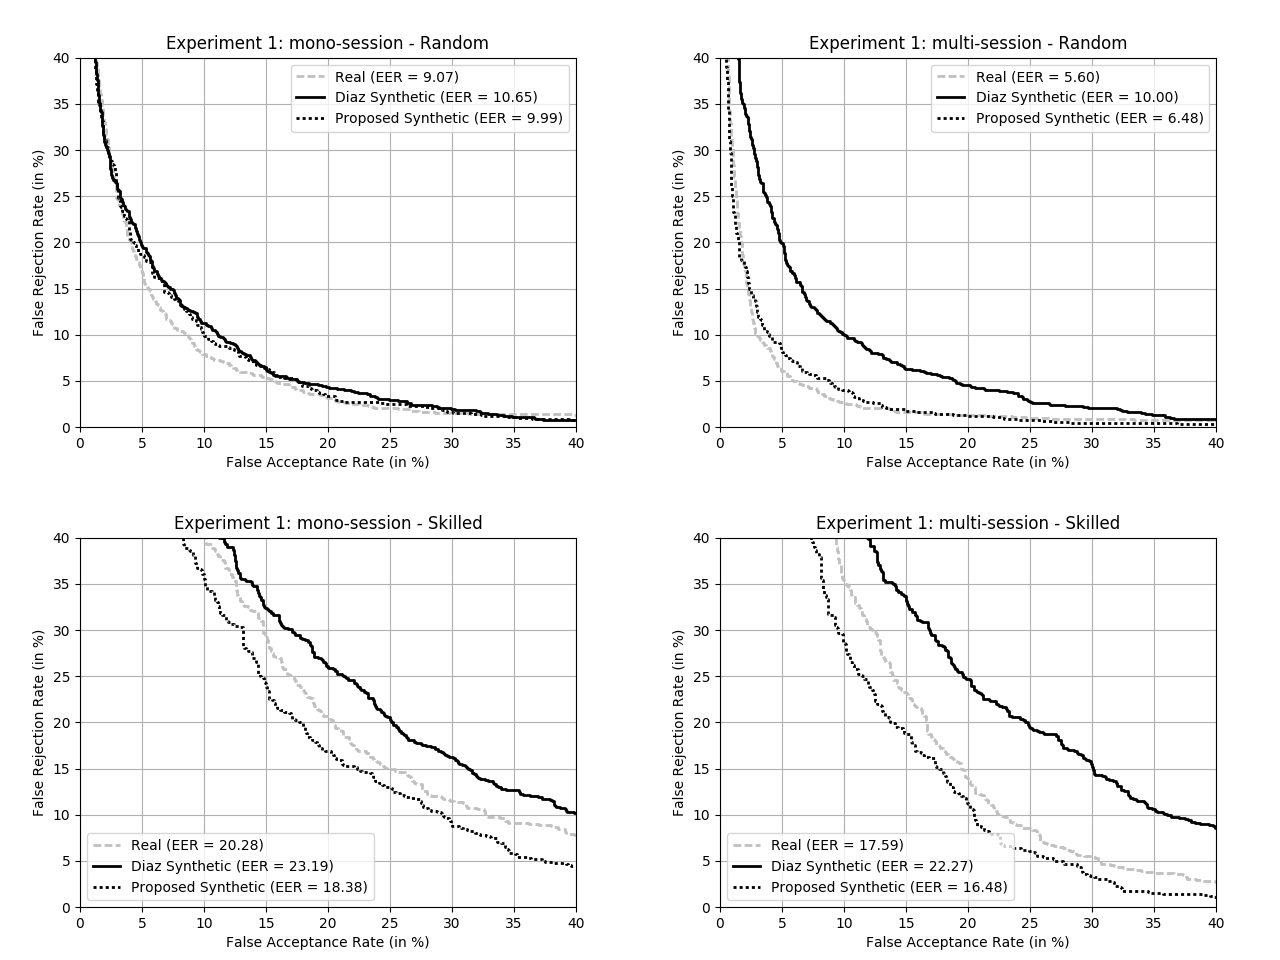
\includegraphics[width=6.6in]{rocs/experiment1}
	% where an .eps filename suffix will be assumed under latex, 
	% and a .pdf suffix will be assumed for pdflatex; or what has been declared
	% via \DeclareGraphicsExtensions.
	\caption{DET curves for real off-line signatures and synthetic signatures (from Diaz and our proposed method), for the first experiment (mono-session and multi-session enrollment), for the two scenarios considered (random and skilled impostors)}
	\label{exp1}
\end{figure*}
\section{Experimental Protocol}
In order to answer the questions stated at the beginning of this section and accomplish a fair comparison of our work and the state of the art, we follow the same experiment protocol proposed by Diaz \cite{diaz2014generation}. Two different experiments are carried out. The Experiment 1 focus on evaluating the synthetic signatures performance in comparison to real signatures and the Experiment 2 evaluates the feasibility of synthetically increasing the number of samples available in a dataset. 

For both experiments the BiosecurID dataset is split into two subsets. The first 90 users are separated as the enrollment set, used to compute the genuine and skilled impostor scores. The remaining 42 authors are considered as the test set and are used to compute the random impostor scores. The performance is evaluated in terms of equal error rate (EER), which is the point in the Detection Error Tradeoff curve (DET) where the false acceptance rate equals the false rejection rate.

\subsection{Experiment 1: synthetic signatures in comparison to real signatures}

Two different protocols have been considered to
compute the 90 user enrolled models:
\begin{inlinelist}
  \item a mono-session approach, using the four samples of the first session
  \item a multi-session approach, using one sample of  each session 
\end{inlinelist}.

In both cases, genuine scores are computed matching the non-enrolled genuine samples of the subject (12) to the enrolled model (90×12 = 1080 genuine scores). Random impostor scores are calculated comparing the first sample of the test subjects to the
enrolled model, leading to 90×42 = 3780 random impostor scores, and skilled impostor scores are calculated with the skilled forgeries samples of the enrolled users
(12 per subject) to the enrolled model (90×12 = 1080 skilled impostor scores).

\subsection{Experiment 2: synthetically increasing the enrollment samples}

This experiment is designed to assess whether synthetically increasing the enrollment dataset leads to a better recognition performance. Three different enrollment sets are considered in this experiment: 
\begin{itemize}
  \item 4 real samples belonging to the
  first acquisition session
  \item 8 real samples belonging to the first and
  the second sessions
  \item 4 real samples belonging
  to the first session plus 4 synthetic samples belonging
  to the second session.
\end{itemize}

\section{Statistical Evaluation}